%%%%%%%%%%%%%%%%%%%%%%%%%%%%%%%%%%%%%%%%%%%%%%%%%%%%%%%%%%%%%%%%%%%%%%%%%
%%%%%%%%%%%%%%%%%%%%%%%%%      INTRODUÇÃO      %%%%%%%%%%%%%%%%%%%%%%%%%%
%%%%%%%%%%%%%%%%%%%%%%%%%%%%%%%%%%%%%%%%%%%%%%%%%%%%%%%%%%%%%%%%%%%%%%%%%

\section{\esp Introdução}

Instituída em 10 de dezembro de 2009, a Lei n.º 12.116/2009 \citeonline{lei}, conforme o Congresso Nacional Brasileiro, decreta o dia 27 de novembro como o Dia Nacional de Luta contra o Câncer de Mama. Além de uma data específica para a luta contra esse câncer, foi criada, em 1990, uma campanha cujo objetivo é conscientizar a população sobre a importância da prevenção e do diagnóstico precoce, o chamado Outubro Rosa.

Causado pela multiplicação rápida e desordenada de células anormais, o câncer pode ocorrer em diversas estruturas do corpo, e quando envolve as células das glândulas mamárias, determina o câncer de mama \cite{incaoquee}. Esse tumor divide a primeira posição com o de pulmão no ranking dos cânceres mais incidentes do mundo, além de ser a doença mais comum entre as mulheres, na qual dados da Organização Mundial de Saúde (OMS) e do Instituto Nacional de Câncer (INCA) apontam que houve por volta de 627 mil mortes por câncer de mama no mundo em 2018, sendo 17,7 mil no Brasil \cite{boletimepidemiologico}.

O diagnóstico prévio dessa doença tem alta significância na contenção do progresso da doença, devido à introdução antecipada do tratamento, que favorece o crescimento das chances de sobrevivência do paciente diagnosticado. Diante disso, existem alguns procedimentos basilares empregados para o diagnóstico dessa doença, tais quais: o exame de toque; exames clínicos; exames de imagens como a mamografia, ultrassonografia ou ressonância magnética; e a confirmação via biópsia.

% Problema Escolhido: já está incluso nesse parágrafo.
De acordo com \citeonline{borchartt}, a mamografia é o exame mais comum para a detecção do câncer de mama, mas apresenta algumas limitações, especialmente para mulheres mais jovens e com o tecido mamário denso. Perante o avanço computacional, a termografia se destaca como uma técnica de diagnóstico não invasiva que permite interceptar diferenças de temperatura em diferentes regiões do corpo através da intensidade da radiação infravermelha. Quando aplicada ao câncer de mama, a termografia se torna uma ferramenta essencial para a detecção prévia da doença. Isso porque as células cancerígenas tendem a apresentar temperaturas mais elevadas do que as células normais, independentemente de fatores como idade e outros \cite{leles}.

% Motivações
Com a evolução da computação em diversos âmbitos tecnológicos, tais como redes neurais, processamento de imagens e inteligências artificiais, oportunidades foram criadas para investigar e implementar soluções avançadas na área da saúde, visando agregar a comunidade médica, além da sociedade no geral. Na oncologia, existem diversos métodos e práticas utilizadas para diagnosticar um quadro de câncer de um paciente, porém, em sua grande maioria, requer uma análise humana que é passiva de erros ou até mesmo incapaz de realizar predições, ou quantificar com precisão o diagnóstico do quadro clínico.

Pautando-se na ideia de trazer ferramentas, compostas por algoritmos avançados que auxiliam médicos no diagnóstico antecipado do câncer de mama, assim melhorando na tomada de decisões dos profissionais de saúde acerca do quadro geral dos pacientes, iniciando tratamento previamente, garantindo uma qualidade de vida e uma longevidade maior para todos assolados pelo quadro de câncer.

% Objetivos
Por meio dos tópicos apresentados, o presente artigo aspira discorrer sobre uma metodologia para o estudo de imagens termográficas, identificando as células como cancerosas utilizando aprendizado por transferência. Outrossim, para investigar de maneira experimental o tema proposto neste artigo, serão empregadas bases de dados, criteriosamente selecionadas e normalizadas em termos de tamanho e histograma, contendo amostras de mamografias para o treinamento de um programa de inteligência artificial a ser desenvolvido. As amostras serão divididas em mamografias sem sinais de câncer, e mamografias com câncer, classificadas de acordo com seus respectivos graus.

Para criar um modelo de classificação de graus, será utilizado o método de \textit{Deep Learning}, que consiste em uma técnica avançada de aprendizado de máquina. Após o treinamento do modelo, sua acurácia será avaliada por meio de testes, e assim que devidamente treinado, o programa será capaz de analisar as imagens dos exames mamográficos e realizar uma classificação precisa e automatizada do câncer de mama, identificando o grau da doença, caso presente no paciente.




%%%%%%%%%%%%%%%%%%%%%%%%%%%%%%%%%%%%%%%%%%%%%%%%%%%%%%%%%%%%%%%%%%%%%%%%%
%%%%%%%%%%%%%%%%%%%      FUNDAMENTAÇÃO TEÓRICA       %%%%%%%%%%%%%%%%%%%%
%%%%%%%%%%%%%%%%%%%%%%%%%%%%%%%%%%%%%%%%%%%%%%%%%%%%%%%%%%%%%%%%%%%%%%%%%


%Informações para contextualizar o leitor.
\section{\esp Fundamentação teórica} 
%9 artigos
% 1.{souza} Souza (2018) - Giovanna
% 2.{noninvasive} Arora (2008) - Giovanna
% 3.{techniques} - CHITRADEVI (2014) - Baesse
% 4.{histopathological} Belsare e Mushif (2012) - Baesse 
% 5.{lungcancer} SHARMA JINDAL (2011) - Baesse
% 6.{machinelearning} UDDIN (2022) - Yago
% 7.{deeplearning} LAUZON (2012) - Yago
% 8.{cnn} ALBAWI (2017) - Yago
% 9.{medical} UMER (2021) - Yago

De modo a fornecer informações mais detalhadas sobre os tópicos vitais para a compreensão do presente artigo, serão retratados conceitos fundamentais sobre o câncer de mama, exames e tratamentos para a doença, bem como técnicas de processamento de imagens termográficas. Além disso, será discutida a técnica de \textit{Deep Learning} com o uso de imagens para demonstrar sua relevância no contexto da detecção do câncer de mama.



%%%%%%%%%%%%%%%%%%%%%%      CÂNCER DE MAMA       %%%%%%%%%%%%%%%%%%%%%%%

\subsection{\esp Câncer de mama}
As células vivas que compõem o corpo humano se dividem para permitir o crescimento e a substituição de células danificadas ou mortas. A proliferação celular é regulada pelos genes do `DNA', transmitidos pelos pais e gerenciados para manter o equilíbrio no processo de divisão celular. O câncer, em geral, se forma quando esse controle genético é danificado ou perdido em uma, ou mais células que então continuam a se dividir normalmente, produzindo mais células anormais, causando danos a outros tecidos e funções corporais \cite{basicOncology}.

% 1.{souza} Souza (2018) - Giovanna
O câncer de mama, em específico, se dá pelo crescimento de células anormais na glândula mamária, e os sub-tipos diferentes desse câncer estão localizados sob o tecido adiposo\footnote{tecido que armazena gordura e mantém a maior reserva de energia do organismo} e no sistema ductal\footnote{ductos responsáveis por conduzir o leite até a papila}. Conforme apontado por \citeonline{souza}, o câncer de mama apresenta células com uma taxa de duplicação de tamanho estimada em 4 meses. Embora o crescimento seja inicialmente lento, quando o tumor se torna palpável e não é tratado, o câncer pode se disseminar para os linfonodos, pulmões, ossos, fígado e cérebro, desenvolvendo metástase.

% 2.{noninvasive} Arora (2008) - Giovanna
A descoberta prévia do câncer de mama aumenta significativamente a probabilidade de um paciente se curar da doença, pendendo de qual método for utilizado para a detecção. Com isso, é necessário avaliar se o método escolhido é invasivo ou não. Outrora ou Dantes, os equipamentos de medição de emissão infravermelha eram capazes de captar uma variação de temperatura apenas de 0,5 a 1 °C, utilizando uma tecnologia primitiva que exigia que um filme de cristal líquido fosse colocado nos seios dos pacientes para detectar a temperatura. Hodiernamente, segundo \citeonline{noninvasive}, as câmeras de termografia infravermelhas digitais conseguem identificar mudanças de 0,08 °C, em adição de não demandar contato físico com o paciente.




%%%%%%%%%%%%%%%%%%%%%%     PROCESSAMENTO DE IMAGEM       %%%%%%%%%%%%%%%%%%%

\subsection{\esp Processamento de Imagem}

% 3.{techniques} - CHITRADEVI (2014) - Baesse
Matematicamente, uma imagem pode ser descrita como uma função bidimensional, f(x, y), onde \textbf{x} e \textbf{y} representam coordenadas espaciais, e a amplitude de \textbf{f} em qualquer par de coordenadas é chamada de a intensidade ou nível de cinza da imagem naquele ponto \cite{techniques}. Quando \textbf{x}, \textbf{y} e os valores de intensidade de \textbf{f} são quantidades finitas e discretas, chamamos a imagem de imagem digital. É essencial que uma imagem digital seja composta por um número finito de elementos (conhecidos como píxeis, \textit{pels} ou elementos de imagem), cada um com sua própria localização e valores específicos. 

% 4.{histopathological} Belsare e Mushif (2012) - Baesse 
% 5.{lungcancer} SHARMA JINDAL (2011) - Baesse
A definição básica de processamento de imagem refere-se ao processo de tratamento de imagens digitais, incluindo a remoção de ruídos e outros tipos de irregularidades presentes \cite{histopathological}. Durante as últimas quatro a cinco décadas, várias técnicas foram desenvolvidas no campo de processamento de imagens, sendo a maioria desenvolvida para aprimorar imagens obtidas por espaçonaves não tripuladas, sondas espaciais e aeronaves militares de reconhecimento. Devido a fácil disponibilidade de computadores poderosos, dispositivos de memória de grande porte e software gráfico, os sistemas de processamentos de imagem estão se tornando cada vez mais populares. Uma das principais vantagens dos métodos de processamento é versatilidade, repetibilidade e preservação da precisão dos dados originais, utilizando técnicas como: \textbf{(i)} Pré-processamento, \textbf{(ii)} Melhoria, \textbf{(iii)} Segmentação, \textbf{(iv)} Extração de recursos, e \textbf{(v)} Classificação \cite{lungcancer}.


% 3.{techniques} - CHITRADEVI (2014) - Baesse
As imagens capturadas por satélites e câmeras convencionais ou digitais carecem de contraste e brilho devido a limitações nos subsistemas de imagem, ou condições de iluminação durante a captura. Além disso, segundo \citeonline{techniques}, essas imagens podem conter diferentes tipos de ruído. Nesse contexto, o aprimoramento de imagem procura acentuar certas características da imagem para análise posterior ou exibição. Os exemplos incluem contraste e retoque de borda, pseudo-coloração, filtragem de ruído, nitidez e ampliação. As técnicas de aperfeiçoamento, que englobam alargamento de contraste, conforme mostrado na \textbf{Figura \ref{fig:figura1}}, modificação do histograma e filtragem de ruído, consoante à \textbf{Figura \ref{fig:figura2}}, são úteis na extração de recursos, análise e exibição. Entretanto, o próprio processo de aprimoramento não aumenta o conteúdo de informações inerentes aos dados, enfatizando somente certas características de imagem especificadas. Algoritmos de aprimoramento são geralmente interativos e dependentes de aplicativos.

 \begin{figure}[ht]
 	\centering	
 	\caption[\hspace{0.1cm}Grade Computacional.]{Alargamento de Contraste}
 	\vspace{-0.4cm}
 	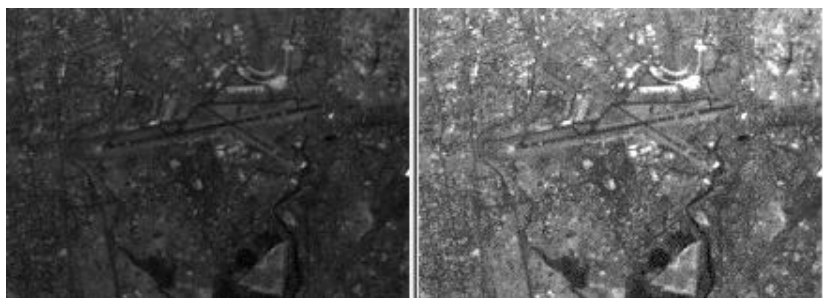
\includegraphics[width=0.6\textwidth]{figuras/Alargamento de Contraste.png}
 	\captionsetup{justification=centering}
	\vspace{-0.2cm}
	\\\textbf{\footnotesize Fonte: \cite{techniques} }
	\label{fig:figura1}
\end{figure}

 \begin{figure}[ht]
 	\centering	
 	\caption[\hspace{0.1cm}Grade Computacional.]{Retirada de Ruido}
 	\vspace{-0.4cm}
 	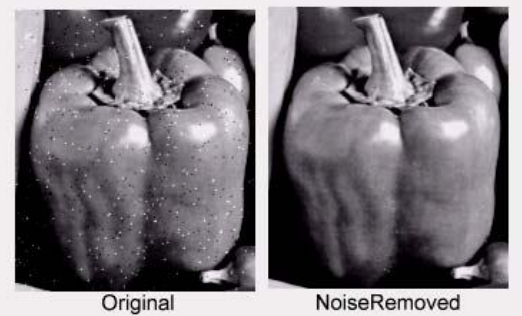
\includegraphics[width=0.6\textwidth]{figuras/Retirada de Ruido.png}
 	\captionsetup{justification=centering}
	\vspace{-0.2cm}
	\\\textbf{\footnotesize Fonte: \cite{techniques} }
	\label{fig:figura2}
\end{figure}



%%%%%%%%%%%%%%%%%%%%%%%%%%     DEEP LEARNING       %%%%%%%%%%%%%%%%%%%%%%

\subsection{\esp Deep Learning}

% 6.{machinelearning} UDDIN (2022) - Yago
\textit{Machine Learning} é um processo que utiliza uma gama de dados para criar uma inteligência artificial instruído para aprender e operar funções de maneira autônoma \cite{machinelearning}. Dentre as abundantes formas de se aplicar esse processo, uma das mais comuns é o método \textit{Deep Learning}, que utiliza redes neurais convolucionais para criar aplicações mais completas. 


% 7.{deeplearning} LAUZON (2012) - Yago
O termo \textit{Deep Learning} refere-se à estrutura utilizada para realização do método, que consiste em várias camadas de neurônios artificiais conectados, permitindo que o sistema aprenda representações cada vez mais complexas dos dados de entrada. Esses dados podem variar desde um simples conjunto de inteiros, para fazer uma predição de cálculo, até um sistema de navegação de um veículo Tesla \cite{deeplearning}.

Os neurônios artificiais são a principal composição da rede neural, sendo estruturas agrupadas em camadas, inspiradas nos neurônios biológicos presentes no cérebro humano. Cada neurônio artificial recebe diversas entradas, representadas por valores numéricos, multiplicadas por um determinado peso e somados. Esse resultado é então processado mediante uma função de ativação, que determina a saída do neurônio, e é transmitida para os outros neurônios da rede.



%%%%%%%%%%%%%%%%%%%%%%%%%%     REDES NEURAIS       %%%%%%%%%%%%%%%%%%%%%%

\subsection{\esp Redes Neurais}


% 8.{cnn} ALBAWI (2017) - Yago
% 9.{medical} UMER (2021) - Yago
A \textit{Convolutional Neural Network} (CNN), de acordo com \citeonline{cnn}, é uma estrutura complexa composta por inúmeros neurônios e camadas de convolução compostas por um conjunto de filtros que, por sua vez, detectam características visuais específicas em uma imagem por meio de uma matriz. Sua arquitetura pode ser dividida em três camadas individuais: \textbf{(i)} \textit{Input Layer} (camada de entrada), \textbf{(ii)} \textit{Hidden Layers} (camadas escondidas), e \textbf{(iii)} \textit{Output Layer} (camada de saída), com funções de entrada, processamento, e saída de dados respectivamente \cite{medical}.

Na camada de entrada (\textit{Input Layer}), os dados brutos, como fotos e vídeos, são recebidos e transformados em dados matemáticos enviados para as camadas seguintes da CNN \cite{cnn}. Nas camadas escondidas (\textit{Hidden Layers}), são usadas funções matemáticas não-lineares modeladas para retornar valores específicos, consoantes os dados de entrada. Esses valores são então enviados para a última parte da rede. Por fim, na camada de saída (\textit{Output Layer}), é produzido o resultado com base nas predições das camadas anteriores.





%%%%%%%%%%%%%%%%%%%%%%%%%%%%%%%%%%%%%%%%%%%%%%%%%%%%%%%%%%%%%%%%%%%%%%%%%
%%%%%%%%%%%%%%%%%%%%      TRABALHOS CORRELATOS       %%%%%%%%%%%%%%%%%%%%
%%%%%%%%%%%%%%%%%%%%%%%%%%%%%%%%%%%%%%%%%%%%%%%%%%%%%%%%%%%%%%%%%%%%%%%%%



%% 1 PARAGRAFO PARA CADA TRABALHO CORRELATO %%
%   Trabalhos com o tema PARECIDO. 
%       Qual o problema que o artigo correlato resolve (cancer de mama, outra doenca)? 
%       Qual o contexto? 
%       O que eles estão propondo? 
%       Estão usando quais técnicas/metodos? 
%       O quão bom foram os resultados que eles tiveram (assertividade ou outras métricas)? 
%
\section{\esp Trabalhos correlatos}
%Usado 1 artigo: 
% 1.{marinePredators} Rajinikanth (2021) - Giovanna
% 2.{comparing} Rodrigues (2014) - Giovanna
% 3.{segmentacao} Baffa (2016) - Giovanna
% 4.{MachineVision} Alberto Martin and Sabri Tosunoglu (2000) - Baesse
% 5.{botelho} Botelho (2007) - Giovanna
% 6.{NakagamiImages} Muhtadi (2022) - Luiza
% 7.{systematic} Systematic Review - Husaini (2020) - Luiza
% 8.{ChaoticSalp} Ibrahim (2020) - Luiza
% 9.{borchartt} Ibrahim (2020) - Luiza
% 10.{leles} leles (2015) - ?
% 11.{ashokkumar} Ashokkumar (2022) - ?

%%%%%%% A FAZER - TRABALHOS CORRELATOS


%%%%%%% COMO REFERENCIAR TRABALHOS CORRELATOS? (exemplos) %%%%%%%

%Utilizando {um método/aplicação/algoritmo} para {ação que o método se propoe a fazer}, \cite{Cite o artigo} obtiveram um resultado de...

%O método para {ação que o método se propoe a fazer} proposto em \cite{Cite o artigo} utilizou...

Neste tópico, serão abordados trabalhos correlatos ao diagnóstico de câncer utilizando inteligência artificial, porém, se diferenciado em termos médicos, como o diagnóstico de outras doenças, em termos de tipo de entrada a ser computada, como radiografias, ou até mesmo imagens digitais. As análises dos trabalhos relacionados também se diferenciarão em termos de abordagem, utilizando-se de outros algoritmos de \textit{Machine Learning}. Além disso, serão feitas analises das propostas dos trabalhos, além dos resultados e assertividades.

% 1.{marinePredators} Rajinikanth (2021)
Em \citeonline{marinePredators}, a avaliação de desempenho é executada e baseada na classificação de acurácia. Ao propor um modelo de detecção de câncer de mama, o trabalho alcançou uma acurácia de 92\%, normalizando as imagens termográficas e utilizando o \textit{Marine-Predators-Algorithm} que auxilia na otimização da seleção das características (definidas por algumas técnicas de reconhecimento de padrões) mais relevantes das imagens e parâmetros do modelo de observação. Para classificar e validar a implementação feita, foram utilizadas variantes (tipos de funções matemáticas que medem a similaridade entre dois pontos no espaço) do algoritmo \textit{Support Vector Machine} (SVM).

% 2.{comparing} Rodrigues (2014) 
Por outro lado, em contraposição ao artigo citado acima,  \citeonline{comparing} ao utilizar outra abordagem de treinamento do algoritmo, chegou em apenas 61,8\% de precisão dos resultados. Foi utilizado o método de limiarização por refinamento adaptativo, técnica que segmenta uma imagem em duas ou mais (com base nos valores dos píxels), de modo que regiões anormais são identificadas com mais precisão. Além disso, o artigo também compara o resultado de entre suas métricas com outros trabalhos referenciados no mesmo, e com base nisso, concluiu-se que a inconsistência das comparações foi devido ao uso de imagens infravermelhas distintas, uma vez que foram utilizadas 102 imagens de uma base de dados pública.
%Diz q usa limiarização baseado na Section III .ASPECTS OF THE APPLIED APPROACH: "In our approach we have used the same methodology that composed the automatic ROI segmentation developed in [19] that was proven to produce good results regarding a comparison to a (...)"

% 3.{segmentacao} Baffa (2016) - Giovanna
Assim como o trabalho acima, \citeonline{segmentacao} utiliza da limiarização por refinamento adaptativo, todavia, com uma acurácia de 96\%. Foram introduzidos três parâmetros para avaliação, baseando-se na informação de que as pregas mamárias (área indicadora de limites inferiores da mama, pois possuem maior temperatura) podem variar de tamanho, dificultando a identificação das mamas. Os parâmetros determinam miliares mínimos de uma área medida em píxels que a prega deve ter, além de definir a área mínima a ser medida em píxel para duas componentes distintas. Com isso, foi possível determinar qual conjunto de parâmetros maximiza as métricas estatísticas apresentadas, determinando assim os resultados normalizados.

% 4.{MachineVision} Alberto Martin and Sabri Tosunoglu (2000) - Baesse
Como aplicado em \citeonline{MachineVision} de modo a desenvolver técnicas de Visão de Máquina, foram utilizados para fundamentação do trabalho a Álgebra de Imagens que forma uma base teórica para dar fundação à implementação de visão computacional, e algoritmos de processamento de imagens. Com o uso de linguagens de alto nível confiáveis e eficientes, inúmeros algoritmos foram otimizados resultando na criação de poderosas ferramentas acessíveis para pesquisadores e cientistas, aumentando a precisão dos resultados. A discussão da visão de máquina básica e algoritmos de processamento de imagem do artigo foram implementados em cinco grupos principais: 
\begin{enumerate}
  \renewcommand{\labelenumi}{\alph{enumi})}
    \item \textbf{Técnicas de Segmentação ou Limiar em \textit{Grey-Level}}: utilizando métodos como \textit{P-tile} (histogramas), \textit{Edge Pixel} e \textit{Interative};
    
    \item \textbf{Técnicas de Detecção de Borda}: localização da borda para aumentar o contraste, utilizando o algoritmo \textit{Canny Edge Detection};
    
    \item \textbf{Morfologia Digital}: filtra a imagem, além de fazer uma análise geométrica da estrutura dos elementos;
    
    \item \textbf{Textura}: observação da repetição de padrões a fim de substitui-los usando \textit{grey level};
    
    \item \textbf{Algoritmos de Esqueletização e Encurtamento}: definir propriedades globais dos objetos e reduzir a imagem em um modelo mais compacto para reconhecer padrões.
\end{enumerate}


% 5.{botelho} Botelho (2007) - Giovanna
Utilizando redes neurais para reconhecer imagens de câncer de pele e unindo técnicas de processamento de imagens digitais, \citeonline{botelho} possibilita a elaboração de um sistema que diferencia imagens de Melanomas. Para isso, quatro características são usadas para identificar uma lesão: assimetria, bordas irregulares, cor variada e diâmetro. Baseadas nessas características, o modelo proposto implementa a rede neural \textit{Perceptron} de Camada Única, utilizando dois neurônios: um excitado por imagens de lesões Melanoma, e outro excitado por imagens de lesões não Melanoma. O Perceptron identifica quando uma entrada é classificada erroneamente e ajusta os pesos por meio de uma regra de correção de erro, conhecida como Regra Delta. Com isso, a rede é treinada somente quando todas as saídas correspondem com a saída esperada, atingindo uma taxa de 69\% de acertos.

% 6. {NakagamiImages} Muhtadi (2022) - Luiza
\citeonline{NakagamiImages} apresenta uma abordagem baseada em \textit{Deep Learning} para detecção e classificação de massas na mama combinando imagens de ultrassom \textit{B-mode} e Nakagami, para fornecer informações complementares sobre o padrão de dispersão de tecidos. O ultrassom B-mode consiste em uma técnica que utiliza ondas sonoras de alta frequência enviadas ao corpo, e refletidas pelos tecidos internos, criando uma imagem em escala cinza aonde as áreas mais brilhantes representam tecidos mais densos. Já as imagens Nakagami são geradas a partir da análise das amplitudes de sinal retornadas pelo tecido examinado, fornecendo informações sobre a presença de diferentes tipos de estruturas. Utilizando uma arquitetura de rede neural convolucional para extrair características das imagens combinadas, as massas são classificadas como malignas ou benignas. Por fim, abordagem proposta foi provada altamente eficaz na localização de massas, com uma precisão de 91,8\%, um desempenho significativamente melhor do que as abordagens existentes que usam apenas imagens B-mode ou Nakagami.

% Esses artigos estão com foco em iamgens termográficas e na acurácia que um banco de dados público pode fornecer:
% 7.{systematic} Systematic Review - Husaini (2020) - Luiza
Em \citeonline{systematic}, são analisados os diferentes tipos de Redes Neurais Artificiais (ANN) e modelos de \textit{Deep Learning} já utilizados na literatura para processar imagens termográficas de câncer de mama. Mesmo que a termografia, conforme o texto, seja atualmente o melhor método para a descoberta precoce, a qualidade das imagens é um desafio tangível. O processo de melhoramento da imagem tenta mostrar detalhes escondidos e destacar características para que a profundidade e tamanho do tumor sejam distinguidos de um tecido saudável. Para melhorar a qualidade da imagem, o trabalho utiliza um dispositivo de resfriamento de mama. Além disso, são destacadas as contribuições e desvantagens de trabalhos relacionados que empregam termografia e inteligência artificial, obtidos mediantes comparações feitas no decorrer do artigo e são desenvolvidos questionamentos a cerca dos desafios enfrentados, como a falta de padronização na aquisição de imagens térmicas e a necessidade de mais dados de treinamento para as redes neurais. 

% 8.{ChaoticSalp} Ibrahim (2020) - Luiza
Para desenvolver uma técnica precisa e eficiente para a identificação antecipada do câncer de mama, \citeonline{ChaoticSalp} usa a segmentação de imagens térmicas em conjunto com o algoritmo \textit{Chaotic Salp Swarm}. O algoritmo proposto consiste em uma técnica de otimização bioinspirada, usada para ajustar os parâmetros de segmentação das termografias e encontrar as regiões suspeitas de câncer de mama. Assim como o anterior, foi utilizada uma base de dados pública de imagens térmicas para avaliar a eficácia do método proposto. Os resultados obtidos foram avaliados baseados em métricas como: sensibilidade, especificidade e coeficiente de Dice. Não é especificado o índice de precisão do trabalho, entretanto, é considerado que o método proposto teve um desempenho satisfatório em termos de precisão na segmentação de regiões suspeitas de câncer de mama nas imagens térmicas.

% 9.{borchartt} Ibrahim (2020) - Luiza
\citeonline{borchartt} teve como foco a análise das potenciais contribuições que o uso de imagens infravermelhas tem para diagnósticos de doenças na mama. Para o estudo, foram utilizadas 102 imagens infravermelhas (IR) de mama única do banco de dados público da Pro Engenharia (PROENG) (sendo 47\% com alguma anormalidade) e resultados foram obtidos através do uso de algoritmos para detecção de condições malignas, como \textit{Support Vector Machine}, para extrair as características como primeiro momento, terceiro momento, não uniformidade da massa cinzenta e porcentagem de execução. Ao longo do texto, é exposta à dificuldade em realizar o processo de segmentação da região da mama, extração da região de interesse, devido à natureza amorfa e a falta de limites claros. Além disso, é apontado que ao usar um banco de dados público para comparar as imagens e extrair características, os melhores resultados foram obtidos com o classificador \textit{Sequential Minimum Optimization} (SMO), em adição a expor a inconsistência da comparação entre trabalhos que utilizam imagens IR. 

% 10.{leles} Leles (2015) 
Buscando explorar métodos não invasivos para a localização precoce do câncer de mama, \citeonline{leles} propõe o uso de imagens térmicas que permitem detectar mudanças na temperatura, causadas pelo aumento do fluxo sanguíneo na área afetada pelo tumor. Após o pré-processamento, foi feito o refinamento manual da região de interesse para que alguns atributos extraídos não colaborassem com dados de fora da mama. Avaliando 70 pacientes, o trabalho identifica a temperatura máxima, mínima e média das mamas para utilizar no cálculo da sensibilidade (capacidade do teste em identificar corretamente o diagnóstico) e especificidade (capacidade do teste em excluir corretamente os que não tem a doença), com os valores de 92,3\% e 86,2\%, respectivamente.

% 11.{ashokkumar} Ashokkumar (2022) 
A fim de abordar a detecção de metástase em linfonodos axilares em pacientes com câncer de mama, \citeonline{ashokkumar} utiliza o método de \textit{Data Augmentation} que faz modificações geométricas das imagens (como rotação, inversão, deslocamento e dimensionamento). Isso fornece uma garantia de que o modelo se concentra em áreas de câncer de mama, em vez de fontes de ruído aleatórias. Conforme o texto, foi demonstrado que o método ajuda na memorização de qualidades específicas das imagens treinadas, e evita que as redes se tornem superajustadas, ou seja, um modelo de aprendizado profundo que se adaptou demasiadamente nos dados de treinamento a ponto de não conseguir capturar padrões mais amplos de novos. Além disso, usando ANN, o trabalho alcançou 98\% de acurácia superando modelos de radiografia.




% \subsection{\esp Inserções de ilustrações}

% As ilustrações devem ser inseridas seguindo o exemplo da Figura \ref{fig:figura1}. 
% % Figura
% \begin{figure}[ht]
% 	\centering	
% 	\caption[\hspace{0.1cm}Grade Computacional.]{Uma Grade Computacional como fonte transparente}
% 	\vspace{-0.4cm}
% 	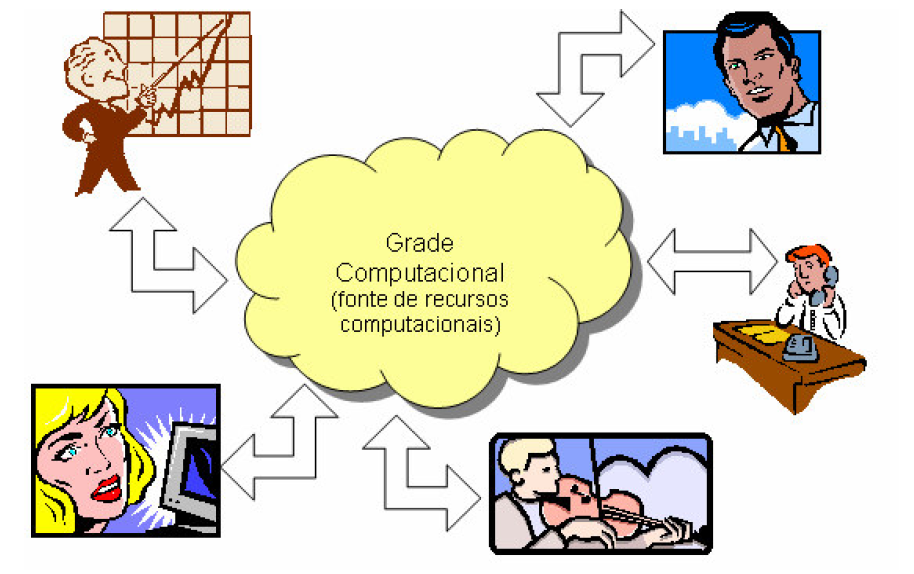
\includegraphics[width=0.6\textwidth]{figuras/grade-comp.png}
% 	% Caption centralizada
% % 	\captionsetup{justification=centering}
% 	% Caption e fonte 
% 	 \vspace{-0.2cm}
% 	\\\textbf{\footnotesize Fonte: \cite{cap-livro} }
% 	\label{fig:figura1}
% \end{figure}
% \vspace{-0.5cm}

% \subsection{\esp Conclusão}
% Discussão dos resultados obtidos na pesquisa. É onde se colocam as observações do autor. 
% Poderá também apresentar sugestões de novas linhas de estudo.
% A conclusão deve estar de acordo com os objetivos do trabalho.
% A conclusão não deve apresentar citações ou interpretações de outros autores.